%\documentclass[color=dvipsnames,handout]{beamer}
\documentclass[color=dvipsnames,aspectratio=169]{beamer}
%\usetheme{plain}
%\usetheme{Singapore}
\usetheme{default}
\usepackage{graphicx}
%\usepackage[dvipsnames]{color}
\usepackage{tikz}
\let\pgfimageWithoutPath\pgfimage
\renewcommand{\pgfimage}[2][]{\pgfimageWithoutPath[#1]{../Figures/#2}}
\usepackage{multirow}
\usepackage{ulem}
\usepackage{xcolor}
%\usepackage{enumitem}
\usepackage{amsthm}
\usepackage{amsmath}
\usepackage{bm}
%\usepackage{fontspec}
\usepackage{amssymb}
%\usepackage{harvard}
\usepackage{natbib}
\usepackage{tabularx,multirow,tabu,booktabs}
\usepackage{transparent}
\newtheorem{thm}{Proposition}%[section]
\newcommand\ov{\overline}
\newcommand\un{\underline}
\newcommand\BB{\mathbb}
\newcommand\EE{\mathbb{E}}
\newcommand\mc{\mathcal}
\newcommand\ti{\tilde}
\newcommand\h{\hat}
\newcommand\beq{\begin{equation}}
\newcommand\eeq{\end{equation}}
\newcommand\barr{\begin{array}}
\newcommand\earr{\end{array}}
\newcommand\bfp{\mathbf{p}}
\newcommand\pder[2]{\frac{\partial #1}{\partial #2}}
\DeclareMathOperator*{\plim}{plim}

\definecolor{back}{HTML}{FFF5EE} %{FFFFF0} %{FDF5E6} %{F5F4EF}
\definecolor{c1}{HTML}{221E1D}
\definecolor{c2}{HTML}{63AA9C}
\definecolor{c3}{HTML}{E9633B}
\definecolor{c4}{HTML}{f5f4ef}
\setbeamertemplate{navigation symbols}{}
\setbeamercolor{title}{fg=c2}
%\setbeamerfont{block title}{series=\boldheadingfont}
\setbeamercolor{block title}{fg=c2}
\setbeamercolor{background canvas}{bg=back}
% \setbeamercolor{caption name}{fg=black}
% %\setbeamerfont{caption}{series=\palatino}
% \setbeamerfont{caption}{size=\footnotesize}
\setbeamercolor{frametitle}{fg=c2,bg=back}
%\setbeamercolor{background canvas}{bg=c4}
\setbeamerfont{normal text}{series=\palatino}
%\setbeamerfont{normal text}{series=\headingfont}
% \setbeamerfont{headline}{series=\headingfont}
% \setbeamerfont{author}{series=\headingfont}
% \setbeamerfont{date}{series=\headingfont}
\setbeamercolor{structure}{fg=c2}
\setbeamercolor{enumerate item}{fg=c2}%{fg=black}
\setbeamercolor{itemize item}{fg=c2}%{fg=black}
\setbeamercolor{itemize subitem}{fg=c2}%{fg=black}
% \setbeamercolor{enumerate item}{fg=black}
\newcommand{\myitem}{\item[-]}
\setbeamertemplate{itemize items}{-}
%\newcommand{\myitem}{\item[$\bullet$]}
\newcommand\eps{\epsilon}
\newcommand\veps{\varepsilon}
\newenvironment{wideitemize}{\itemize\addtolength{\itemsep}{10pt}}{\enditemize}

\title{\large ECON4261 - Quasi-Experiments: The Child Penalty}
\author{Joseph Mullins}
\date{}

\begin{document}

\frame{\titlepage}


\frame{\frametitle{Introduction}
    \begin{wideitemize}
        \item The paper: \emph{Children and Gender Inequality: Evidence from Denmark} by Kleven, Landais, and S\o gaard. {\it American Economic Journal: Applied Economics}, 2019, 11(4) \pause
        \item Background: fertility is thought to be a major driver of wage gaps (recall facts from the CPS on this!)
        \begin{itemize}
            \item Reductions in experience
            \item Effects promotions
            \item Statistical discrimination
            \item Selection into occupation
        \end{itemize} \pause
        \item Paper estimates the {\color{c3}``child penalty''} - the effect of birth of the first child on earnings and employment - and uses some descriptive methods to explore potential mechanisms.
    \end{wideitemize}
}

\frame{\frametitle{Methodology Part (1): Raw Estimates}
    Main specification for person of gender $g$ at event-time $t$ and year $s$
    \[ Y^{g}_{ist} = \sum_{j\neq -1}{\color{c3}\alpha^{g}_{j}}\mathbf{1}\{j=t\} + \sum_{k}\beta^g_{k}\mathbf{1}\{k=age_{is}\} + \sum_{y}\gamma^{g}_{y}\mathbf{1}\{y=s\} + \nu^{g}_{nst} \] \pause
    Notes:
    \begin{itemize}
        \item $t=0$ is the year of first (the ``event'') for each individual
        \item Model is identified from variation in the {\color{c3}timing} of the first birth \pause
        \item     Convert $\alpha^{g}_{t}$ to a percentage effect by calculating:
        \[ P^{g}_{t} = \frac{\alpha^{g}_{t}}{\EE\left[ \sum_{k}\beta^g_{k}\mathbf{1}\{k=age_{is}\} + \sum_{y}\gamma^{g}_{y}\mathbf{1}\{y=s\} \right]} \]
    
    \end{itemize}
}

\frame{\frametitle{Methodology Part (2): Decomposition}
Allow for differences in the child penalty by year:
\[ Y^{g}_{ist} = \sum_{y}\sum_{j\neq -1}{\color{c3}\alpha^{g}_{yj}}\mathbf{1}\{j=t\}\mathbf{1}\{y = s\} + \sum_{k}\beta^g_{k}{\color{c2}X_{kns}}  + \nu^{g}_{nst} \] \pause
and decompose the wage gap into potential sources in year $s$:
\[ \Delta_{s} = \mathbb{E}[\alpha^{m}_{st}-\alpha^{w}_{st}|s] + \sum_{k}(\beta^{m}_{k} - \beta^{f}_{k})\EE[X^{m}_{kns}] + \sum_{k}\beta^{w}_{k}\EE[X^{m}_{kns} - X^{w}_{kns}]  \]
{\color{c3}Important:} $X_{kns}$ must not be anything that can be affected ``downstream'' causally by childbirth. Think pre-birth measures of investment such as education and initial occupation.
}

\frame{\frametitle{Results}
\begin{center}
    \vspace{-30pt}
    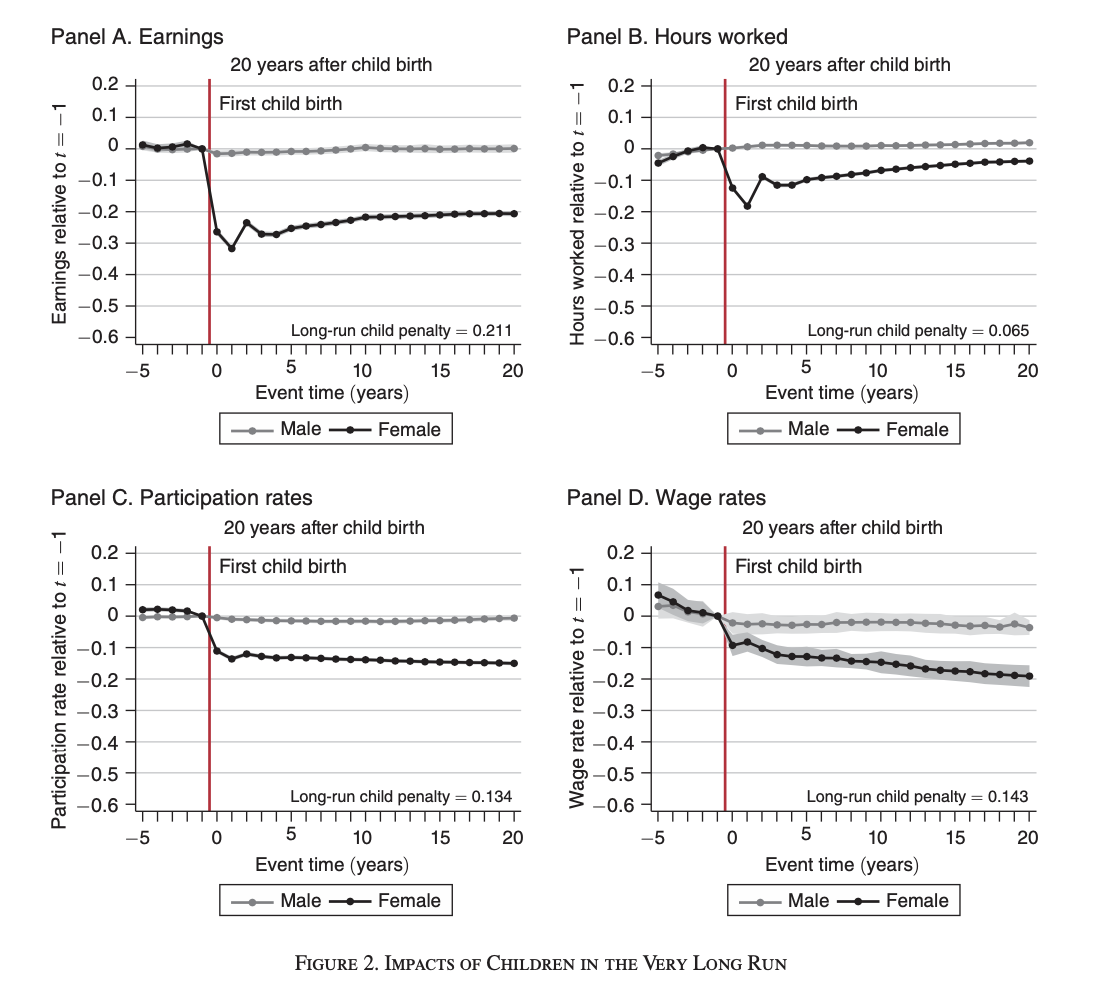
\includegraphics[scale=0.5]{../figures/Kleven1.png}
\end{center}
}

\frame{\frametitle{Results}
\begin{center}
    %\vspace{-30pt}
    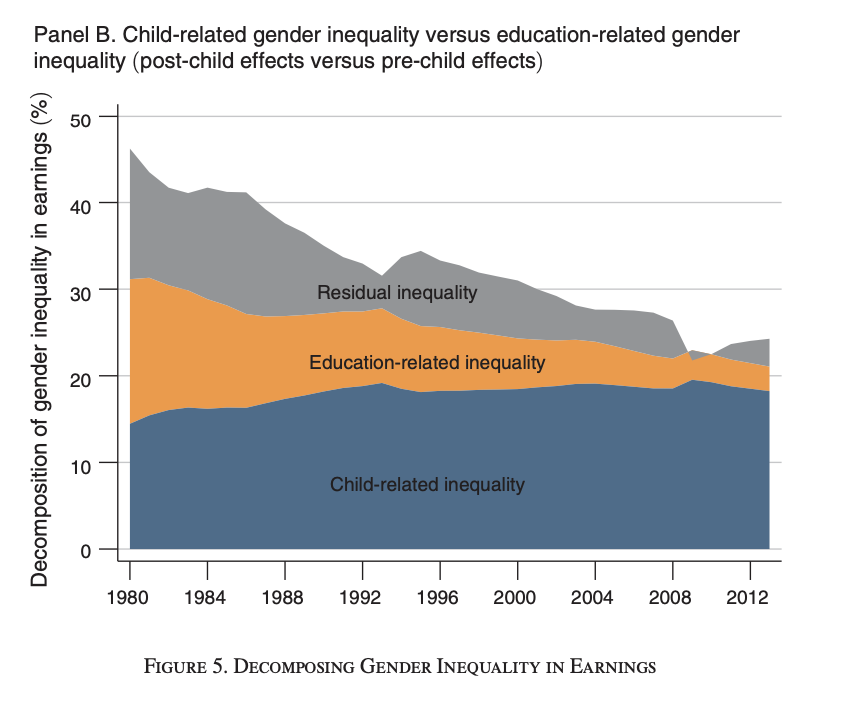
\includegraphics[scale=0.6]{../figures/Kleven2.png}
\end{center}
}


\frame{\frametitle{Robustness}
They test their estimates of the child penalty two ways:\vspace{10pt}
\begin{wideitemize}
    \item Extend the data to include individuals who never have children. These are used to form a control group in a difference-in-difference estimator. {\color{c3}Same results}.
    \item Compare the model's estimates of the effect of birth of a third child to IV estimates of the effect using the gender ratio of the first two children as an instrument. {\color{c3}Same results}.
\end{wideitemize}
}

\frame{\frametitle{Last Exercise}
The authors estimate penalties separately by relative work experience of maternal and paternal grandparents. \pause
\begin{center}
    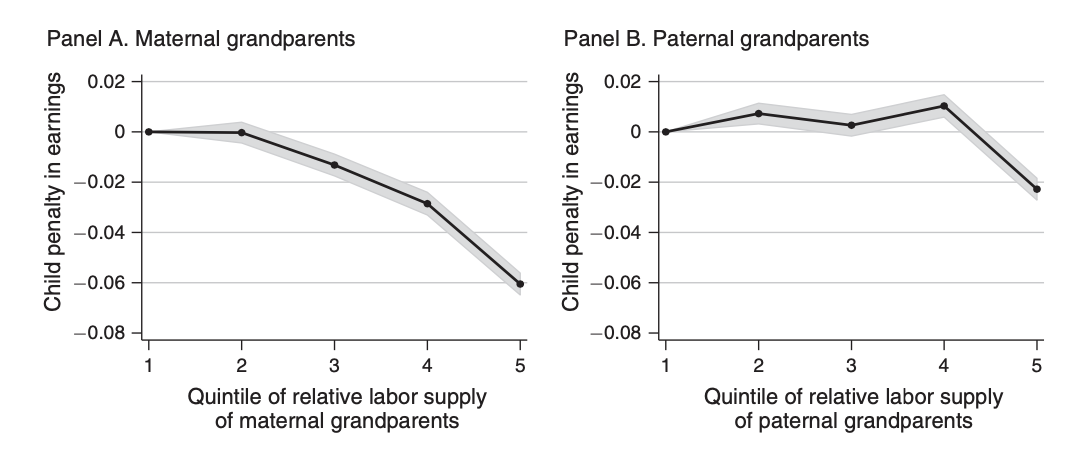
\includegraphics[scale=0.5]{../figures/Kleven3.png}
\end{center}
Suggests some kind of {\color{c2}intergenerational mechanism}.
}

\frame{
    \frametitle{Two Comments}
    \begin{wideitemize}
        \item In general I find the resuls quite convincing, but...
        \item The model estimates imply that the first child has a positive effect on outcomes for women in the 5 years prior. This seems fishy and they don't comment on it at all. \pause
        \item When you don't normalize by the outcome variables, the raw effects are quite big for men as well as for women (will see this in recitation). No comment on this. Do we believe those results also? \pause
        \item Selection on timing of first birth could be driving all the results.
    \end{wideitemize}
}


\end{document}
